\documentclass{tikzposter} % See Section 3

\usepackage[nolinks]{qrcode}
\usepackage{natbib}
\usepackage{mciteplus}
\usepackage[T1]{fontenc}
\usepackage{fontspec}
\usepackage{xcolor}
\usepackage{amssymb}
\definecolor{orange}{rgb}{1,0.5,0}
\definecolor{violet}{rgb}{0.58,0,0.827}
\definecolor{jgu}{RGB}{190, 0 , 39}

\usepackage{amsmath}

% funny items
\DeclareFontFamily{U}{skulls}{}
\DeclareFontShape{U}{skulls}{m}{n}{ <-> skull }{}
\newcommand{\skull}{\text{\usefont{U}{skulls}{m}{n}\symbol{'101}}}
\newcommand{\good}{\item[{\color{orange}$\bigstar$}]} 
\newcommand{\bad}{\item[{\color{violet}$\skull$}]} 
\newcommand{\ugly}{\item[{\color{red}$\bigstar/\skull$}]} 

% modifying the color of the title background
\definecolorstyle{myColorStyle}{
	\colorlet{titlebgcolor}{jgu}
}{}


% eliminate the Bibliography title
\renewcommand{\bibsection}{}

\title{Retention Time Alignment}
\institute{University Medical Center, Johannes Gutenberg University, Germany}
\author{Mateusz Krzysztof Łącki, Ute Distler, Stefan Tenzer}
% \titlegraphic{
\includegraphics{img/jgu.jpeg}}
\usetheme{Simple} % See Section 5
\usetitlestyle{Filled}
\usecolorstyle{myColorStyle}

% redoing the title section
% \settitle{ 

% 	
\includegraphics{img/jgu.jpeg}
% 	\centering \vbox{
%      [\TP@titlegraphictotitledistance] \centering
%      \color{titlefgcolor} {\bfseries \Huge \sc \@title \par}
%      \vspace*{1em}
%      {\huge \@author \par} \vspace*{1em} {\LARGE \@institute}
% }
% 	\qrcode[hyperlink,height=5in]{https://github.com/MatteoLacki/rta}
% }

\makeatletter
\newcommand\insertlogo[2][]{\def\@insertlogo{\includegraphics[#1]{#2}}}
\newcommand\insertqr[2][]{\def\@insertqr{\qrcode[hyperlink,height=#1]{#2}}}

\newlength\LogoSep
\setlength\LogoSep{0pt}

\insertlogo[width=10cm]{img/jgu3.pdf}
\insertqr[3in]{https://github.com/MatteoLacki/rta}

\renewcommand\maketitle[1][]{  % #1 keys
    \normalsize
    \setkeys{title}{#1}
    % Title dummy to get title height
    \node[transparent,inner sep=\TP@titleinnersep, line width=\TP@titlelinewidth, anchor=north, minimum width=\TP@visibletextwidth-2\TP@titleinnersep]
        (TP@title) at ($(0, 0.5\textheight-\TP@titletotopverticalspace)$) {\parbox{\TP@titlewidth-2\TP@titleinnersep}{\TP@maketitle}};
    \draw let \p1 = ($(TP@title.north)-(TP@title.south)$) in node {
        \setlength{\TP@titleheight}{\y1}
        \setlength{\titleheight}{\y1}
        \global\TP@titleheight=\TP@titleheight
        \global\titleheight=\titleheight
    };
    % Compute title position
    \setlength{\titleposleft}{-0.5\titlewidth}
    \setlength{\titleposright}{\titleposleft+\titlewidth}
    \setlength{\titlepostop}{0.5\textheight-\TP@titletotopverticalspace}
    \setlength{\titleposbottom}{\titlepostop-\titleheight}

    % Title style (background)
    \TP@titlestyle

    % Title node
    \node[inner sep=\TP@titleinnersep, line width=\TP@titlelinewidth, anchor=north, minimum width=\TP@visibletextwidth-2\TP@titleinnersep]
        at (0,0.5\textheight-\TP@titletotopverticalspace)
        (title)
        {\parbox{\TP@titlewidth-2\TP@titleinnersep}{\TP@maketitle}};

    % \node[inner sep=0pt,anchor=west] 
    %   at ([xshift=-\LogoSep]title.west)
    %   {\@insertlogo};
	\node[right of=title, node distance=-.38\titlewidth]
      {\@insertlogo};

    % \node[inner sep=0pt,anchor=east] 
    %   at ([xshift=\LogoSep]title.east)
    %   {\@insertqr};

    \node[left of=title, node distance=-.38\titlewidth, fill=white]
      {\@insertqr};

    % Settings for blocks
    \normalsize
    \setlength{\TP@blocktop}{\titleposbottom-\TP@titletoblockverticalspace}
}
\makeatother

% \settitle{ \centering \vbox{
%      \@titlegraphic \\[\TP@titlegraphictotitledistance] \centering
%      \color{titlefgcolor} {\bfseries \Huge \sc \@title \par}
%      \vspace*{1em}
%      {\huge \@author \par} \vspace*{1em} {\LARGE \@institute}
%      
\includegraphics{img/jgu.jpeg}
% }}


\begin{document}
\maketitle

\begin{columns}
\column{0.5}


\block{Rationale}{
	\begin{itemize}
		\good LC-IM-MS instruments identify thousands of peptides obtained from digested proteins
		\bad most observed signals are not easily sequenced and are useless in the identification process
		\good one can retrieve a lot of unidentified singals by x-annotation!
	\end{itemize}
	\begin{tikzfigure}
		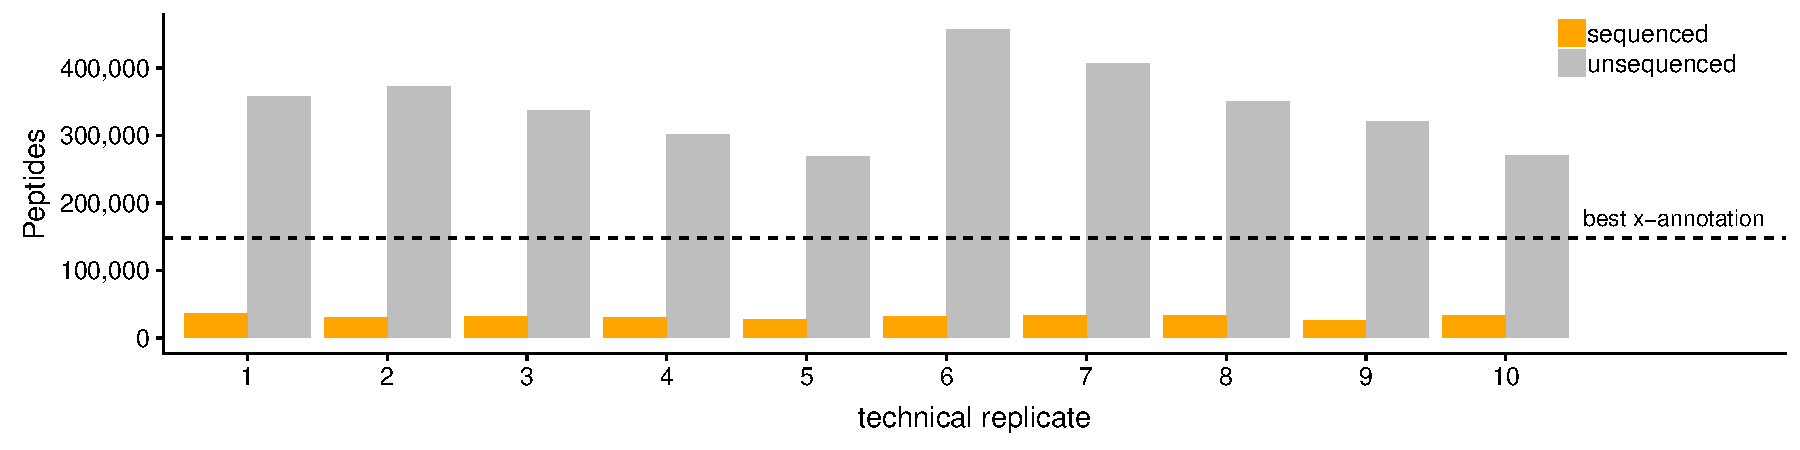
\includegraphics[width=\linewidth]{R/img/x-annotation.pdf}
	\end{tikzfigure}

	\begin{itemize}
		\ugly technical replicates reveal not always the same peptides
		\good biochemical properties of signals in different runs are similar
	\end{itemize}
	
	\begin{tikzfigure}
		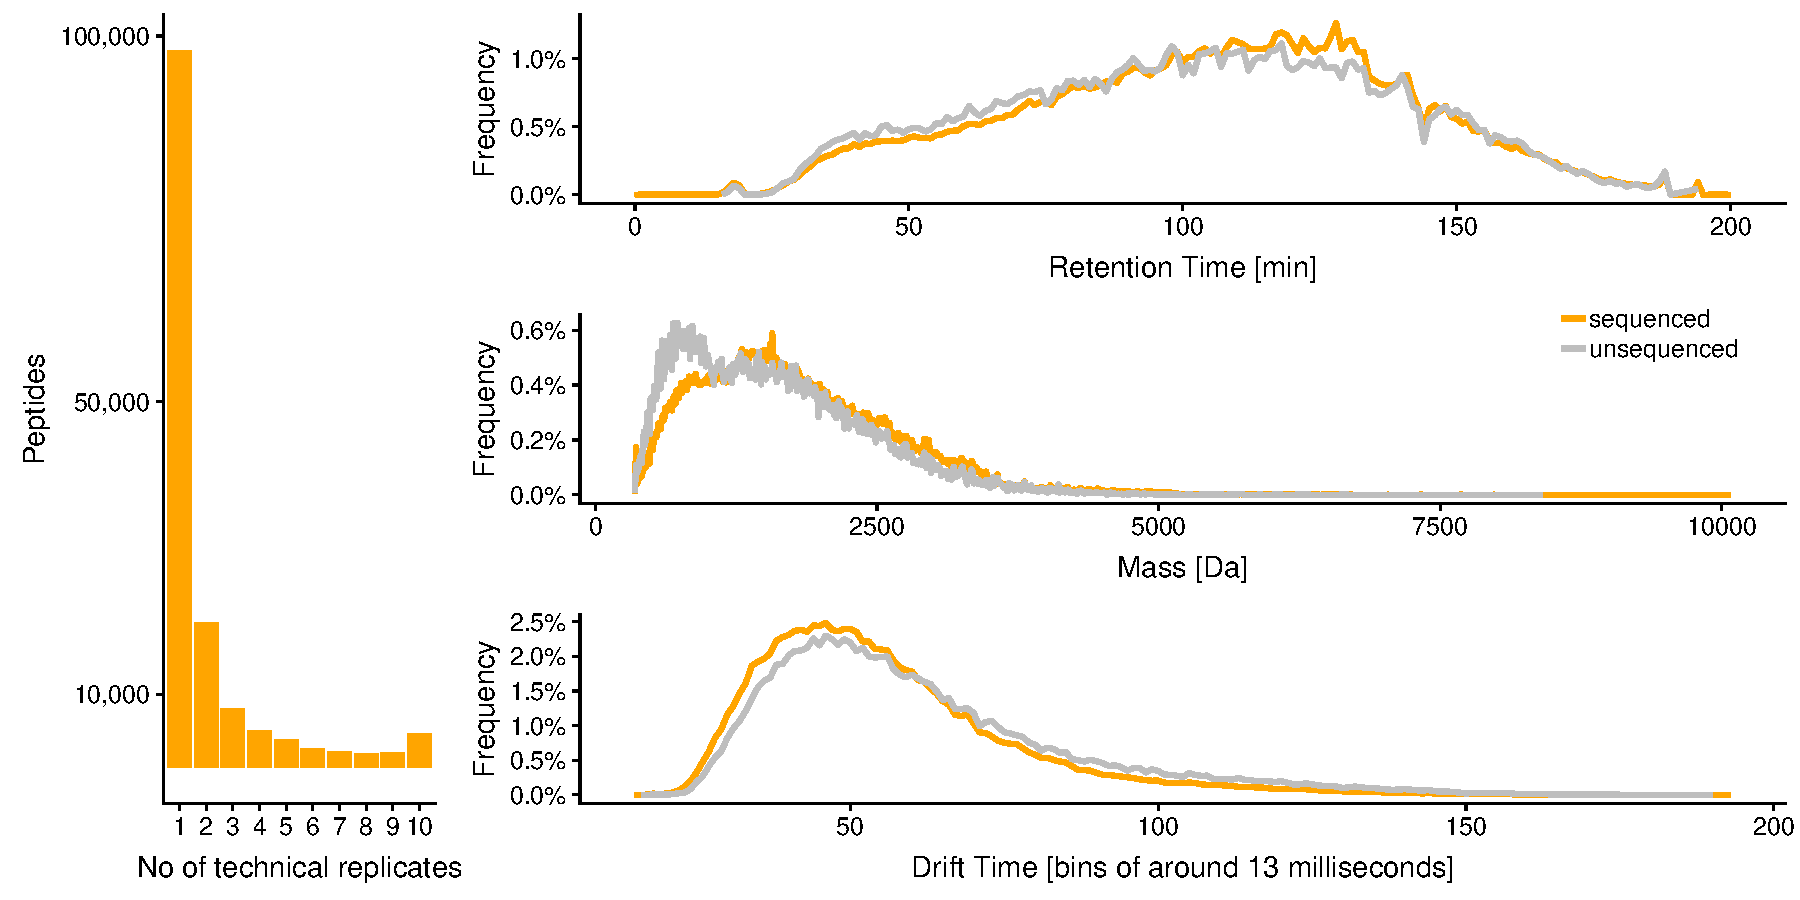
\includegraphics[width=\linewidth]{R/img/venn_and_similarfeatures.pdf}
	\end{tikzfigure}

	\begin{itemize}
		\bad retention times accross technical replicates do show significant systematic deviations
		\bad some sequenced peptides differ significantly between runs
	\end{itemize}

	\begin{tikzfigure}
		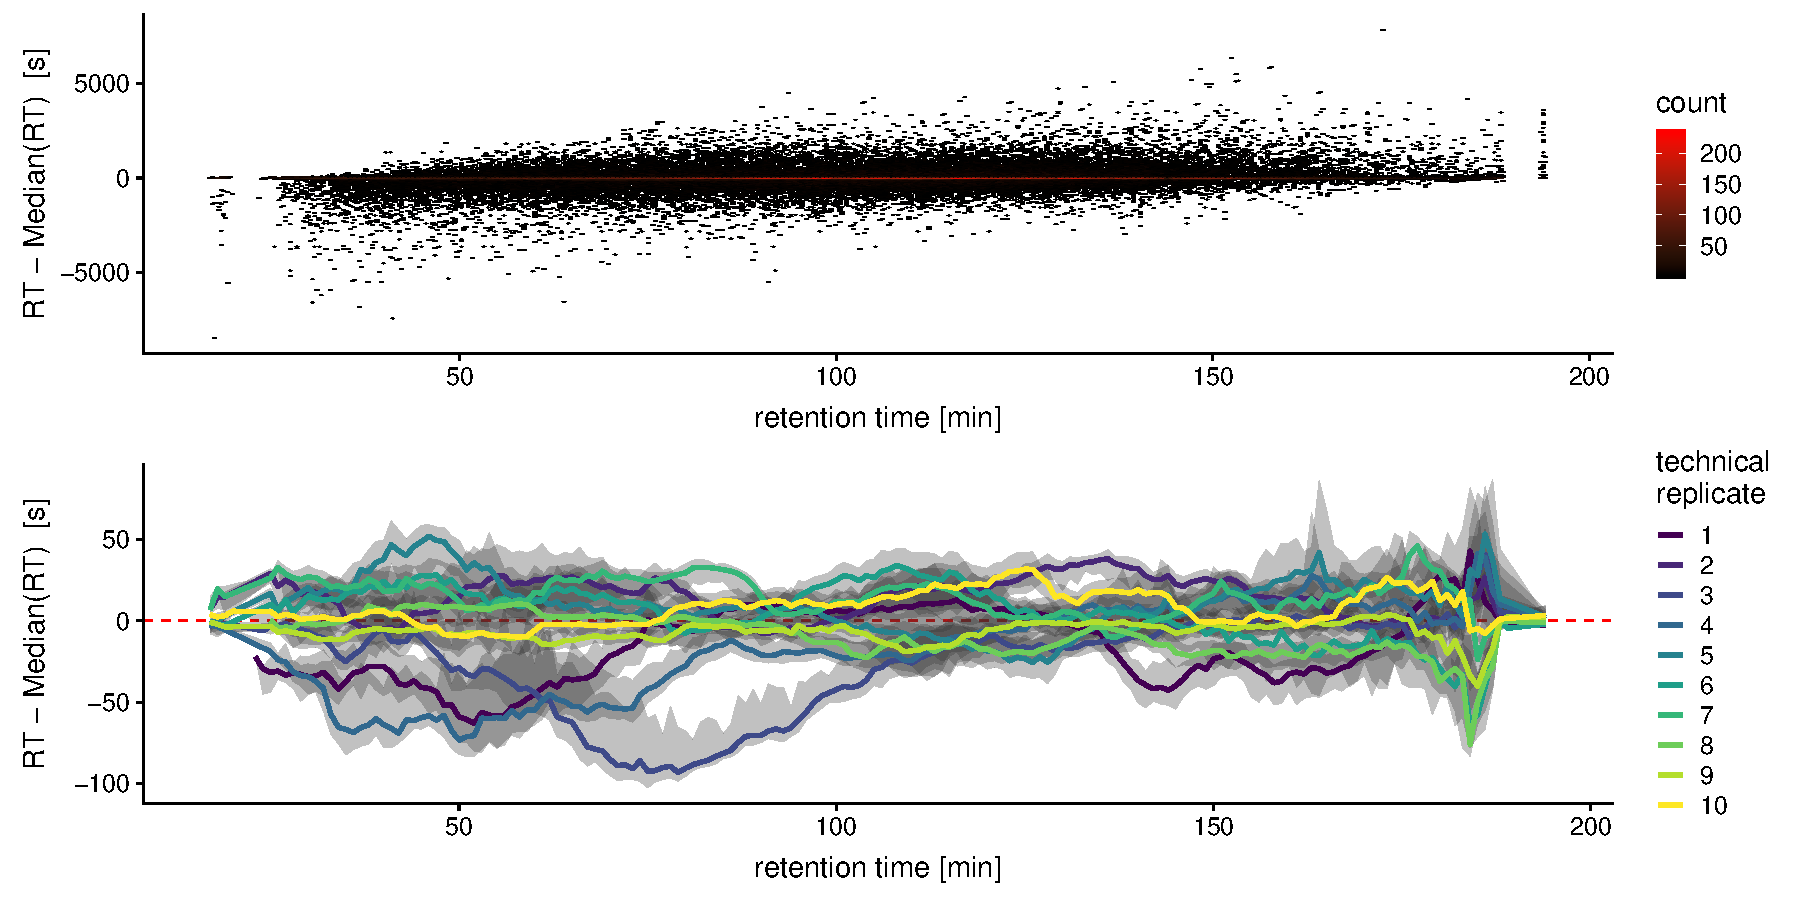
\includegraphics[width=\linewidth]{R/img/rt_dists.pdf}
	\end{tikzfigure}
} 

\block{Retention Time Alignment to the rescue}{
	Brag about the RTA.
}



\column{0.5}




\block{Other similar approaches}{
	The idea of the retention times alignment is not new.
	The \texttt{Match Between Runs} has been a standard part of the \texttt{Max Quant} software\cite{tyanova2016maxquant}.
}

\block{Literature}{
	\bibliographystyle{plain}
	\bibliography{bib/spectrometry}
}
\end{columns}

%\note{Notetext} % See Section 4.3
\end{document}
